%\section{Platform design}

We aim at providing  an open
design to ease contributive developments from both course authors
and software developers, allowing teachers and researchers to
capitalize and share in an effective manner on e-learning tools and
experiences.

{\em E-learning material description:}
We engineer our Question Answering system with XML
technologies. The first motivation is to help authors to describe effectively
their e-learning material to the platform (figure \ref{arch}).
XML technologies indeed allow a clean separation between  the descriptions of:
(a) the exercises structure (i.e. how exercises are organized into questions,
how questions are connected  with the answers and with the course material),
(b) the presentation itself (i.e. how exercises look like on the screen),
(c) the answers validation process (i.e. how answers are evaluated),
(d) the processing of the XML descriptions themselves (structure
filtering and transformations).
Moreover many related software tools are currently available and
continuously maintained in the open source community, which helps not
to reinvent the wheel. The way we are using XML is the
following.

\begin{figure}[htbp]
{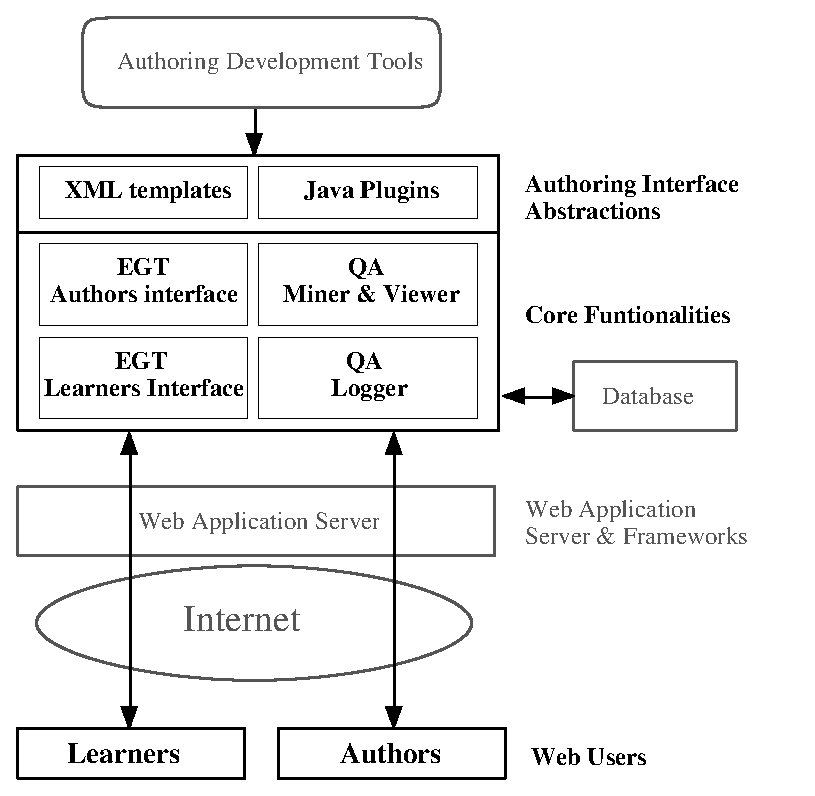
\includegraphics[width=9cm]{arch.eps}}
\caption{The LeVinQuam platform architecture overview.}
\label{arch}
\end{figure}

{\em Data input validation:}
The structure and contents of exercises, e-learning
guided tours and answers  are described in XML in the platform ({\bf EGT} blocks in the synopsis of figure \ref{arch}).
The use of a schema language for XML, as \textsc{Relax NG}, allows an
automatic validation of the exercises descriptions submitted by 
authors by matching these descriptions to an XML schema. The same
process can apply to student answers, once translated into XML in the
platform. The link between exercises and answers can also be made
explicit by means of XML syntax. Logical data input validation is a
fundamental mean for ensuring a reliable processing of these data.

%MS dans ce qui suit, on n'explique pas assez les composants de la
%figure sur l'architecture

{\em Authoring interfaces:}
The platform layer does not pretend to offer to authors an exhaustive
set of graphical-oriented authoring tools, which would represent a
full development project per se.  This is why authoring tools appear
at the top, outside the core area in  figure \ref{arch}.
In contrast we propose to bridge the gap between authors, developers
and the platform by providing an effective set of {\em authoring
interfaces} allowing them to enrich the platform with their own
extensions, letting them define new exercises types, new answers
validators, and further new graphical-oriented authoring tools to help
in these tasks.
%To provide a reliable extension framework, allowing and
%encouraging teachers and researchers to capitalize and share
%contributive developments in an effective manner, robust and open
%standards like XML and Java will be used as root technologies (even if
%rapid application development complements can be further plugged
%in). These authoring interfaces are based on concepts of {\em XML templates} and {\em java plug-ins}.

%MS la phrase pr�c�dente n'est-elle pas un peu redondante avec avant
%et... la suite?
%PD ok, vu.

In a first phase, authors, with the help of a simple
validating XML editor,  fill XML templates describing their
exercises and answers. A template library providing simple generic
types of exercises is proposed to the authors for this purpose. 
%We think
%that XML is simple enough to be quickly mastered by authors because it
%focuses on structure and contents (by contrast, HTML mixes informal
%logic and presentation style).
%Nevertheless, the
%development of authoring tools is encouraged thanks to XML playing the
%role of a common language for interfacing with the core platform.
In a second phase graphical-oriented authoring tools extensions to the
platform  propose to authors a user-friendly environment for
designing exercices and  output the necessary XML data for the
underlying platform authoring interfaces. In both cases, the platform
handles the code generation required to put the exercices on line,
whatever method has been employed by authors for their description.

%\footnote{It can also handle the XML validation
%by means of predefined schemas, like kinds of questionnaires, or, in
%the contrary, infer a schema from an unconstrained XML.}.

{\em Answer validation:}
Different levels of answer validation can be provided by the platform,
according to the nature  of exercises, from syntactic validation,
like checking whether an answer is a valid calendar date, to complex
semantic validations, going through  simple semantic validation of
closed questionnaires, e.g. checking whether 
this date is the correct answer. If the question is to solve a
mathematical equation, then a simple semantic validation can
decide whether the solution is the one expected. However if we want to
analyze and validate more complex formulas, a third level of validation is
necessary, that can only be based on software code having knowledge of the application
field.
To allow authors to provide such validation codes in a robust and
effective way a Java plug-in API is supplied by the platform ({\em Java Plug-in} block in figure \ref{arch}).
For example, in the SQL case study previously mentioned, when a student
answer is an SQL query, a Java plug-in validator would send this query to a
dedicated SQL server and analyse the server's reply (here, from the standpoint of the platform,
Java is a wrapper for SQL).
We  advocate for  the usage of Java within
LeVinQam for several reasons. One of them is the huge collection of Java source code
available on the internet. Portability is also enhanced with Java, which is
a main-stream programming language. Another reason is more
technical: the ease of maintenance, compared with scripting languages,
and the richness of web frameworks based on J2EE (e.g. the java projects at {\tt apache.org}).
%MS r�f�rences 
%% We actually plan to run our platform by means of Java
%% servlets with the support of Tomcat and build the web application with
%% help of open source frameworks, like Struts and Cocoon. These
%% technologies offer a clean architectural and functional model (called
%% Model-View-Controller) and reach a wide audience among companies.

%We previously mentionned an example with SQL and this lead us to
%another aspect of the platform: data persistence. 

{\em Data persistence:}
The last feature of the platform is data persistence. All answers as well as the log of the learner's
interaction with the platform are stored in a relational  database for further data-mining
({\em QA Logger} and {\em QA Miner~\&~Viewer} in figure \ref{arch}).
We  use  XML
transformations to map exercises, answers and guided tours to
the relational database schema.

Most of the aforementioned features, especially layers of answer
validation and data persistence, have been experimented in a first
prototype \cite{wargon01} based on Ganesha \cite{ganesha}.

%MS reference de Ganesha et de laurent Wargon
%This enables further data mining to discover new informations
%and gives some feedback to the teacher. 


%% A trail is a path among the course or the exercises which is proposed
%% to the learner. There can be predefined trails like beginner's trails
%% or advanced trails, but also unconstrained trails which allow the
%% learner to progress freely. These trails can be specified as an XML
%% schema. In all cases, the interactions of the learner along his trail
%% is recorded in the platform database for future mining.

